\documentclass[otchet]{SCWorks}
\usepackage{preamble}

\begin{document}

\chair{математической кибернетики и компьютерных наук}
\title{Базовые команды AviSynth и их использование для монтажа видео}
\course{1}
\group{151}
\napravlenie{09.03.04 "--- Программная инженерия}
\author{Чиженькова Егора Алексеевича}
\date{2026}

\maketitle

\tableofcontents

\intro
AviSynth "--- это скриптовый фреймсервер: файл с расширением \texttt{.avs}
описывает цепочку фильтров, применяемых к видеопотоку, а результат
передаётся любой программе, умеющей открывать видео~\cite{avisynth}.
Собственного графического интерфейса AviSynth не имеет: его роль заключается
в том, чтобы вычислять кадры по требованию, не создавая промежуточных
файлов.

В качестве внешней программы выступает VirtualDub2: он открывает скрипт как
обычный видеофайл, позволяет просмотреть результат и выполнить финальное
кодирование~\cite{virtualdub}. Такая связка покрывает типичные задачи
монтажа домашнего видео: вырезание фрагментов, обрезку краёв кадра,
изменение разрешения и частоты кадров.

Ниже рассматриваются модель фреймсервера, базовые команды AviSynth
и соотношения, связывающие параметры монтажа со свойствами видеопотока,
а также приводится пример конвейера обработки.


\section{Теоретические сведения}

\subsection{Модель фреймсервера}
Скрипт AviSynth "--- это программа, результатом которой является клип:
последовательность кадров с аудиодорожкой. Внешнее приложение запрашивает
у скрипта кадры по требованию, поэтому для него скрипт неотличим от
обычного видеофайла~\cite{avisynth}: фильтры применяются до внутренних
преобразований оболочки и без записи промежуточных данных на диск.

Каждая функция принимает клип и возвращает новый, поэтому вызовы
выстраиваются в цепочку. Если клип не указан явно, он берётся из
специальной переменной \texttt{last}, в которой хранится результат
предыдущей операции.

\subsection{Кадры, длительность и монтаж}
Видеопоток характеризуется частотой кадров $f$ (кадр/с). Номер кадра,
соответствующий моменту времени $t$ (с), вычисляется по формуле (1):
\begin{equation}
N = \lfloor t \cdot f \rfloor .
\end{equation}
Монтаж в AviSynth ведётся в номерах кадров, а не в метках времени: функция
\texttt{Trim(a, b)} оставляет кадры с $a$ по $b$ включительно, поэтому
длительность фрагмента в кадрах равна
\begin{equation}
N_{trim} = b - a + 1 .
\end{equation}
Соотношения (1) и (2) позволяют переходить от длительности фрагмента
в секундах к аргументам функции \texttt{Trim} и обратно~\cite{avisynth}.

\subsection{Масштабирование и ядро Ланцоша}
Изменение разрешения выполняется функцией \texttt{LanczosResize}. В её
основе лежит свёртка с ядром Ланцоша, обеспечивающим более высокую чёткость
по сравнению с билинейной интерполяцией за счёт меньшего размытия на
границах объектов~\cite{lanczosres}:
\begin{equation}
L(x) =
\begin{cases}
\operatorname{sinc}(x) \cdot \operatorname{sinc}\!\left(\dfrac{x}{a}\right), & \text{если } |x| < a, \\
0, & \text{иначе},
\end{cases}
\end{equation}
где $\operatorname{sinc}(x) = \dfrac{\sin(\pi x)}{\pi x}$, а параметр $a$
(обычно $a = 3$) задаёт ширину окна. Формула (3) объясняет, почему
\texttt{LanczosResize} даёт резкую картинку, но может создавать ореолы на
контрастных границах.

\section{Практическое использование}

\subsection{Пример скрипта}
Типовой сценарий подготовки ролика: открыть файл, вырезать фрагмент,
убрать чёрные полосы, уменьшить разрешение и задать точную частоту кадров.
Соответствующий скрипт приведён в листинге 1.

\inputminted{text}{code/AviSynthScript.avs}

Комментарии начинаются с символа \verb|#| и игнорируются интерпретатором.
Для открытия контейнеров MP4 и MKV вместо \texttt{AviSource} применяется
функция \texttt{FFVideoSource} после загрузки плагина FFMS2 командой
\texttt{LoadPlugin}~\cite{ffms2}: встроенная \texttt{AviSource} понимает
лишь AVI с установленными VFW-кодеками~\cite{avisynth}.

\subsection{Базовые функции}
Функции, использованные в листинге 1, сведены в таблицу 1.

\begin{table}[H]
  \centering
  \small
  \begin{tabular}{|l|l|l|}
    \hline
    Функция & Назначение & Пример вызова \\
    \hline
    \texttt{FFVideoSource} & открыть видео любого контейнера & \texttt{FFVideoSource("clip.mkv")} \\
    \texttt{AviSource} & открыть AVI с VFW-кодеком & \texttt{AviSource("clip.avi")} \\
    \texttt{Trim} & оставить диапазон кадров & \texttt{Trim(120, 240)} \\
    \texttt{Crop} & обрезать края кадра & \texttt{Crop(0, 200, 0, -200)} \\
    \texttt{LanczosResize} & изменить разрешение & \texttt{LanczosResize(1280, 720)} \\
    \texttt{ConvertToYV12} & перевести в формат YV12 & \texttt{ConvertToYV12()} \\
    \texttt{AssumeFPS} & задать частоту кадров & \texttt{AssumeFPS(24000, 1001)} \\
    \hline
  \end{tabular}
  \caption{Базовые функции AviSynth}
\end{table}

\subsection{Связка с VirtualDub2}
Скрипт \texttt{.avs} открывается в VirtualDub2 как обычный видеофайл
(File "--- Open video file); окно программы с загруженным скриптом показано
на рисунке 1.

\begin{figure}[H]
  \centering
  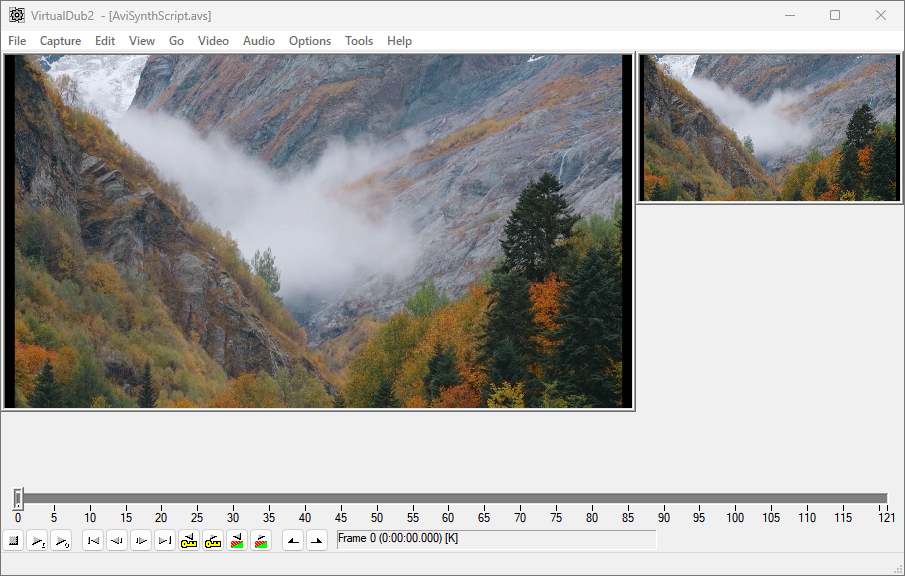
\includegraphics[width=0.9\textwidth]{images/openedscript.png}
  \caption{Скрипт AviSynthScript.avs, открытый в VirtualDub2}
\end{figure}

Дальнейшая обработка выполняется в одном из трёх режимов
(таблица 2).

\begin{table}[H]
  \centering
  \begin{tabular}{|l|l|}
    \hline
    Режим & Когда применяется \\
    \hline
    Direct stream copy & поток копируется без перекодирования \\
    Fast recompress & перекодирование без применения фильтров \\
    Full processing mode & полное применение фильтров и преобразований \\
    \hline
  \end{tabular}
  \caption{Режимы обработки видео в VirtualDub2~\cite{virtualdub}}
\end{table}

Результат работы фильтров кадрирования и масштабирования показан на
рисунке 2: слева "--- исходный кадр с чёрными полосами, справа "--- кадр
после применения \texttt{Crop} и \texttt{LanczosResize}.

\begin{figure}[H]
  \centering
  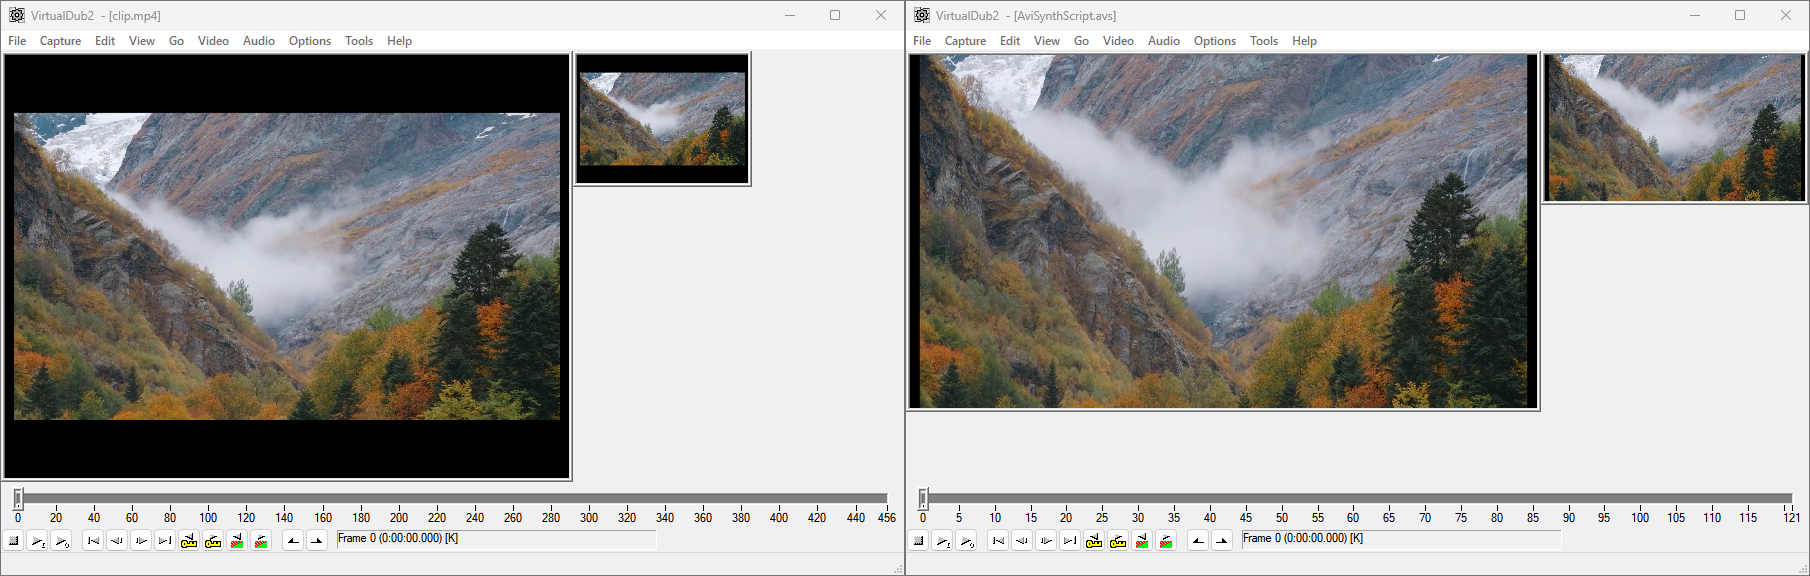
\includegraphics[width=0.96\textwidth]{images/beforeandafter.png}\hfill
  \caption{Кадр до и после применения фильтров кадрирования и масштабирования}
\end{figure}


\conclusion
В ходе работы был рассмотрен подход к обработке видео на основе скриптового
фреймсервера AviSynth в связке с VirtualDub2. Модель фреймсервера, при
которой скрипт отдаёт кадры по требованию внешней программы, определяет
главное преимущество связки перед графическими видеоредакторами:
воспроизводимость~\cite{avisynth}. Один раз написанный текстовый скрипт
гарантирует, что цепочка фильтров будет применена идентично на любой
машине, а отсутствие промежуточных файлов сокращает объём дисковых
операций.

Компактность синтаксиса AviSynth делает его удобным инструментом пакетной
обработки видеоархивов, где ручная настройка каждого ролика
нецелесообразна~\cite{avisynth}. VirtualDub2 в этой связке берёт на себя
роль окна предпросмотра и фронтенда финального кодирования, наследуя
проверенный набор режимов обработки оригинального
VirtualDub~\cite{virtualdub}. Таким образом, пара «код + легковесный GUI»
обеспечивает контроль над качеством и эффективность базового монтажа.


\bibliographystyle{ugost2003}
\bibliography{thesis}

\appendix

\end{document}
